\chapter{Gestures Identified as Appropriate for this Application}
The main type of gesture used by this project is voice recognition. Listed below is the available voice commands you can use as well as what they should accomplish when said. 

\section{Gestures Used and Built Into Alexa}

\begin{enumerate}
    \item Phrase said: What is X?
    \begin{itemize}
    \item Asking "What is" followed by the name of a game will return back various basic information about the game asked. Example: What is Fallout 3?.
    \end{itemize}
    
    \item Phrase said: Who is X?
    \begin{itemize}
    \item Asking "Who is" followed by the name of a character from a game will return back various basic information about said character asked. Example: Who is Master Chief?
    \end{itemize}
    
    \item Phrase said: What is X (Location)?
    \begin{itemize}
    \item Asking "What is" followed by the name of a location from a game will return back various basic information about the location asked. Example: what is Megaton?
    \end{itemize}
\end{enumerate}

\begin{figure}[h!]
    \begin{center}
        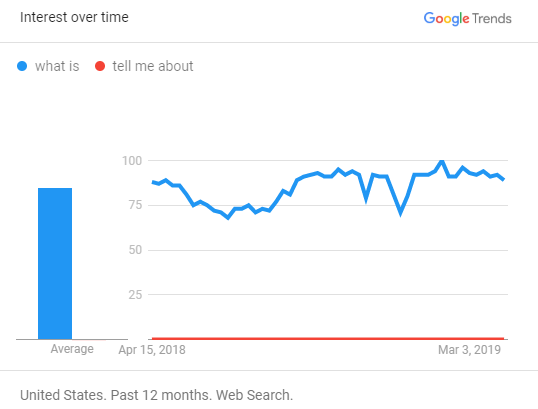
\includegraphics[width=10cm,height=10cm,keepaspectratio]{whatIsStat.png}
        \caption{Who is vs Tell me about}
        \label{fig:gameintent}
    \end{center}
\end{figure}


As you can see from the above picture during out research into what gestures we would use we looking into Google Trends to compare likely gesture that would be used by users. Using Google Trends we compared multiple gestures we thought the user might use on our Alexa skill. We compared what we thought would be the most likely option which was 'What is x?'. We then compared this gesture to others such as 'Tell me about x', in order to figure out which would be the most natural to ask our skill. Out of all the options 'What is x?' was by far the most used to ask Google a question and therefor seemed the most natural to use for our Skill.

\section{Alexa Understanding Gestures not Built-in}
Alexa works by intent, an Alexa intent works like a function would in a programming language. The intent has slots attached to it, these slots work like parameters given to the function. Intents are called by asking the skill to do a task with a given object. 'What is Fallout 3'. 'What is' is the intent and 'Fallout 3' is the object. We give the intent the 'Fallout 3' object which is laid out in the intent as a slot name. With this slot name and the given intent we can run some some of functionality.

With Alexa you program in the intents you wish Alexa to create. But Alexa works by figuring out which of the intents best match what the user is looking to use. Examples of this are 'Alexa what is Fallout 3' and 'Alexa tell me about Fallout 3'. Even though we didn't program in the intent to handle 'Tell me about' Alexa is still able to figure out which intent better matches the phrase by the user.

Tested Phrases:
\begin{enumerate}
    \item Phrase said: About X?
    \begin{itemize}
    {\item \color{green} Successful}
    \item The skill returned the information even thought the gesture wasn't built into the skill
    \end{itemize}
    
    \item Phrase said: Tell me about X?
    \begin{itemize}
    {\item \color{green} Successful}
    \item The skill returned the information even thought the gesture wasn't built into the skill
    \end{itemize}
    
    \item Phrase said: Information for x?
    \begin{itemize}
    {\item \color{green} Successful}
    \item The skill returned the information even thought the gesture wasn't built into the skill
    \end{itemize}
    
    \item Phrase said: What is x and y?
    \begin{itemize}
    {\item \color{red} Failure}
    \item This gesture was too much for the intent as it had no intent that took in two slots. This is akin to calling a function which takes in one string but instead giving it two.
    \end{itemize}
\end{enumerate}

Alexa is extremely robust in its functionality to figure out which intent best suites what the user is asking. This allowed users who had different ways of asking a question to user our skill during testing.

The gesture we built into the skill were very adjustable due to how Alexa tries to understand user intent.
